\documentclass[14pt, a4paper]{report}
\usepackage{mathtext}
\usepackage[T2A]{fontenc}
\usepackage[utf8]{inputenc}
\usepackage[russian]{babel}
\usepackage{multirow}
\usepackage{slashbox}
\usepackage{makecell}
\usepackage{graphicx}
\usepackage{physics}
\usepackage{amstext}
\usepackage{caption}
\usepackage{subcaption}
\usepackage{mathrsfs}

\renewcommand{\thesection}{\arabic{section}.}
\renewcommand{\thesubsection}{\arabic{section}.\arabic{subsection}.}
\newcommand{\EDS}{\ensuremath{\mathscr{E}}}

\title{\textbf{Отчет о выполнении лабораторной работы 2.1.1 "Измерение удельной теплоемкости воздуха при постоянном давлении"}}
\author{Калашников Михаил, Б03-205}
\date{}

\begin{document}
\maketitle

\textbf{Цель работы:}
измерить повышение температуры воздуха в зависимости от мощности подводимого тепла и расхода при стационарном течении через трубу; исключив тепловые потери, по результатам измерений определить теплоёмкость воздуха при постоянном давлении.
\newline

\textbf{В работе используются:}
\begin{itemize}
\item теплоизолированная стеклянная трубка;
\item электронагреватель;
\item источник питания постоянного тока;
\item амперметр, вольтметр (цифровые мультиметры);
\item термопара, подключенная к микровольтметру;
\item компрессор;
\item газовый счётчик;
\item секундомер

\end{itemize}

\section{Теоретические сведения}

Теплоёмкость тела в некотором процессе определяется как их отношение:
\[C=\frac{\var Q}{\dd T}\]

Рассмотрим газ, протекающий стационарно через трубу постоянного сечения, в которой установлен нагревательный элемент. Пусть за некоторое время $\dd t$ через калориметр прошла малая порция газа массой $\dd m=q\dd t$, где $q$ -- массовый расход газа в трубе. Если мощность нагрева равна $N$, мощность тепловых потерь на обмен с окружающей средой $N_{пот}$, то порция получила тепло $\var Q=(N-N{пот})\dd t$. С другой стороны, по определению теплоёмкости: $\var Q=c\dd m\Delta T$, где $\Delta T$ -- приращение температуры газа, $c$ -- удельная (на единицу массы) теплоёмкость газа в рассматриваемом процессе. При малых расходах газа и достаточно большом диаметре трубы можно пренебречь перепадом давления и считать процесс изобарическим. Таким образом, получаем:
\[c_p=\frac{N-N_{пот}}{q\Delta T}\]

\section{Экспериментальная установка}

\begin{figure}[!ht]
\centering
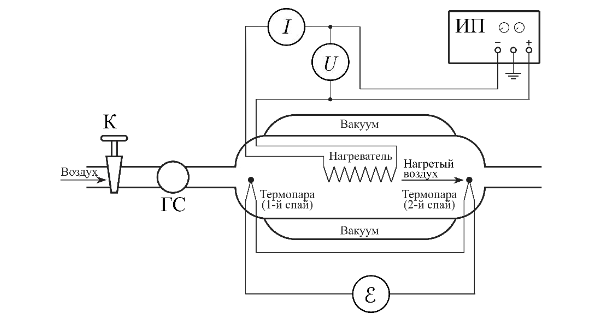
\includegraphics[scale=0.6]{terma8_01.png}
\caption{Экспериментальная установка}
\end{figure}

Схема установки изображена на рис. 1. Воздух, нагнетаемый компрессором, прокачивается через калориметр. Калориметр представляет собой стеклянную цилиндрическую трубку с двойными стенками, запаянными с торцов. Нагреватель в виде расположен внутри калориметра непосредственно в воздушном потоке. Нагрев проволоки производится от регулируемого источника постоянного тока. Напряжение $U$ на нагревателе и ток $I$ через него регистрируются цифровыми мультиметрами. Таким образом, мощность нагрева равна:
\[N=UI\]

Для измерения разности температур $\Delta T$ служит медно-константановая термопара. Один спай термопары расположен в струе воздуха, входящего в калориметр, и находится при комнатной температуре, а второй — в струе выходящего нагретого воздуха. Константановая проволока термопары расположена внутри калориметра, а медные проводники подключены к цифровому вольтметру. Возникающая в термопаре ЭДС $\EDS$ пропорциональна разности температур $\Delta T$ спаев: 
\[\EDS=\beta\Delta T,\quad\beta=40,7\ \frac{мкВ}{^\circ C}\]

Объём воздуха, прошедшего через калориметр, измеряется газовым счётчиком ГС. Для регулировки расхода служит кран К. Массовый расход может быть найден как $q=\rho_0\frac{\Delta V}{\Delta t}$, где $\rho_0$ -- плотность воздуха.
Учитывая мощность тепловых потерь ($N_{пот}=\alpha\Delta T$), можно получить уравнение, описывающее связь подводимой мощности и разноси температур:
\[N=(c_pq+\alpha)\Delta T\]

\section{Проведение эксперимента}

\begin{enumerate}

\item Подготовим к работе газовый счетчик, убедимся в его работоспособности.

\item Убедимся в том, что калориметр охлажден до комнатной температуры, продув его с помощью компрессора.

\item Включим вольтметры и амперметр.

\item Зафиксируем показания температуры и давления в лаборатории: 
\[t_0=21,9\ ^\circ C,\quad P_0=1000,8\ гПа\]

\item Определим максимальный расход газового счетчика. Он равен $5\ л/30\ c$. Сопротивление проволоки нагревателя равно $R_{н}=29\ Ом$. С помощью этих данных можно оценить силу тока $I_0$, необходимую чтобы нагреть воздух на $\Delta T_0=1\ ^\circ C$:
\[I_0=\sqrt\frac{N_0}{R_н}=\sqrt\frac{c_p\rho_0q\Delta T_0}{R_н}\approx83\ мА\]

\item Проведем измерения зависимости разности температур от мощности нагрева $\Delta T(N)$ для значения расхода $q_1$, близкого к максимальному. Постепенно повышая силу тока, пропускаемого через нагревательный элемент, и выжидая между измерениями время, достаточное для установления термодинамического равновесия между термопарой и потоком воздуха, получим несколько значений. Занесем их в таблицу 1. Само же значение расхода может быть определено с помощью секундомера по формуле: $q=\frac{5\ л}{t}$. $t_1=39,2\pm0,3\ с$, $q_1=151\pm1\ \frac{мг}{с}$.

\item После окончания серии измерений охлаждим калориметр до комнатной температуры.

\item Повторим измерения для другого значения расхода воздуха: $t_2=91,4\pm0,5\ с$, $q_2=64,8\pm0,4\ \frac{мг}{с}$.

\item Выключим источник питания, охладим калориметр до комнатной температуры.

\end{enumerate}

\section{Обработка данных}

\begin{enumerate}

\setcounter{enumi}{10}

\item Построим график зависимости $\Delta T(N)$ для каждого расхода воздуха. Видно, что зависимость может быть аппроксимирована прямой. Проведем через точки прямую МНК и найдем угловые коэффициенты $k$:
\[k_1=4,7\pm0,3 \frac{^\circ C}{Вт},\quad k_2=8,7\pm0,5 \frac{^\circ C}{Вт}\]

\item Используя полученные данные, определим значения $c_p$ и $\alpha$:
\[c_p=\frac{1/k_1-1/k_2}{q_1-q_2},\quad \varepsilon_{c_p}=\sqrt{\frac{\sigma_{k_1}^2k_2^4+\sigma_{k_2}^2k_1^4}{(k_1k_2(k_1-k_2))^2}+\frac{\sigma_{q_1}^2+\sigma_{q_2}^2}{(q_1-q_2)^2}}=15\%\]
\[\alpha=\frac{q_1/k_2-q_2/k_1}{q_1-q_2},\quad \varepsilon_{\alpha}=\sqrt{\frac{q_2^2k_2^4\sigma_{k_1}^2+q_1^2k_1^4\sigma_{k_2}^2}{(k_1k_2(q_1k_1-q_2k_2))^2}+\frac{(k_1-k_2)^2(q_2^2\sigma_{q_1}^2+q_1^2\sigma_{q_2}^2)}{((q_1-q_2)(q_1k_1-q_2k_2))^2}}=18\%\]
\[c_p=1,02\pm0,15\ \frac{Дж}{г\cdot{^\circ C}}\]
\[\alpha=49\pm9\ \frac{мВт}{^\circ C}\]

Определим величину теплопотерь $N_{пот}/N$:
\[\frac{N_{пот}}{N}=\frac{\alpha\Delta T}{(c_pq+\alpha)\Delta T}=\frac{1}{1+c_pq/\alpha},\quad\varepsilon_{\frac{N_{пот}}{N}}=\frac{\sqrt{\varepsilon_{c_p}^2+\varepsilon_q^2+\varepsilon_\alpha^2}}{1+\alpha/c_pq}\]
\[\left(\frac{N_{пот}}{N}\right)_1=24\pm4\%,\quad\left(\frac{N_{пот}}{N}\right)_2=42\pm6\%\]

\end{enumerate}

\section{Вывод}

Табличное значение удельной теплоемкости воздуха -- $c_{p0}=1,03\ \frac{Дж}{г\cdot{^\circ C}}$, что попадает в пределы погрешности. Это говорит об успешном выполнении лабораторной работы.

\section{Приложения}

\begin{table}[!ht]
\centering
\makebox[\textwidth][c] {
\begin{tabular}{| c | c | c | c | c | c | c | c | c | c | c |}
\cline{1-5}\cline{7-11}
\multicolumn{5}{| c |}{$q_1=151\ мг/с$} & & \multicolumn{5}{ c |}{$q_2=64,8\ мг/с$} \\
\cline{1-5}\cline{7-11}
$I,\ мА$ & $U,\ В$ & $N,\ Вт$ & $\EDS,\ В$ & $\Delta T,\ ^\circ C$ & & $I,\ мА$ & $U,\ В$ & $N,\ Вт$ & $\EDS,\ В$ & $\Delta T,\ ^\circ C$ \\
\cline{1-5}\cline{7-11}
122,0 & 3,508 & 0,428 & 86 & 2,11 & & 89,2 & 2,558 & 0,228 & 84 & 2,06 \\
\cline{1-5}\cline{7-11}
199,7 & 5,747 & 1,148 & 216 & 5,31 & & 121,6 & 3,492 & 0,425 & 141 & 3,46 \\
\cline{1-5}\cline{7-11}
210,3 & 6,054 & 1,273 & 245 & 6,02 & & 152,1 & 4,370 & 0,665 & 220 & 5,41 \\
\cline{1-5}\cline{7-11}
215,0 & 6,183 & 1,329 & 258 & 6,34 & & 199,9 & 5,742 & 1,148 & 375 & 9,21 \\
\cline{1-5}\cline{7-11}
218,4 & 6,282 & 1,372 & 269 & 6,61 & & 216,3 & 6,218 & 1,345 & 465 & 11,4 \\
\cline{1-5}\cline{7-11}
\end{tabular}
}
\caption{Результаты проведенных измерений}
\end{table}

\begin{figure}[!ht]
\centering
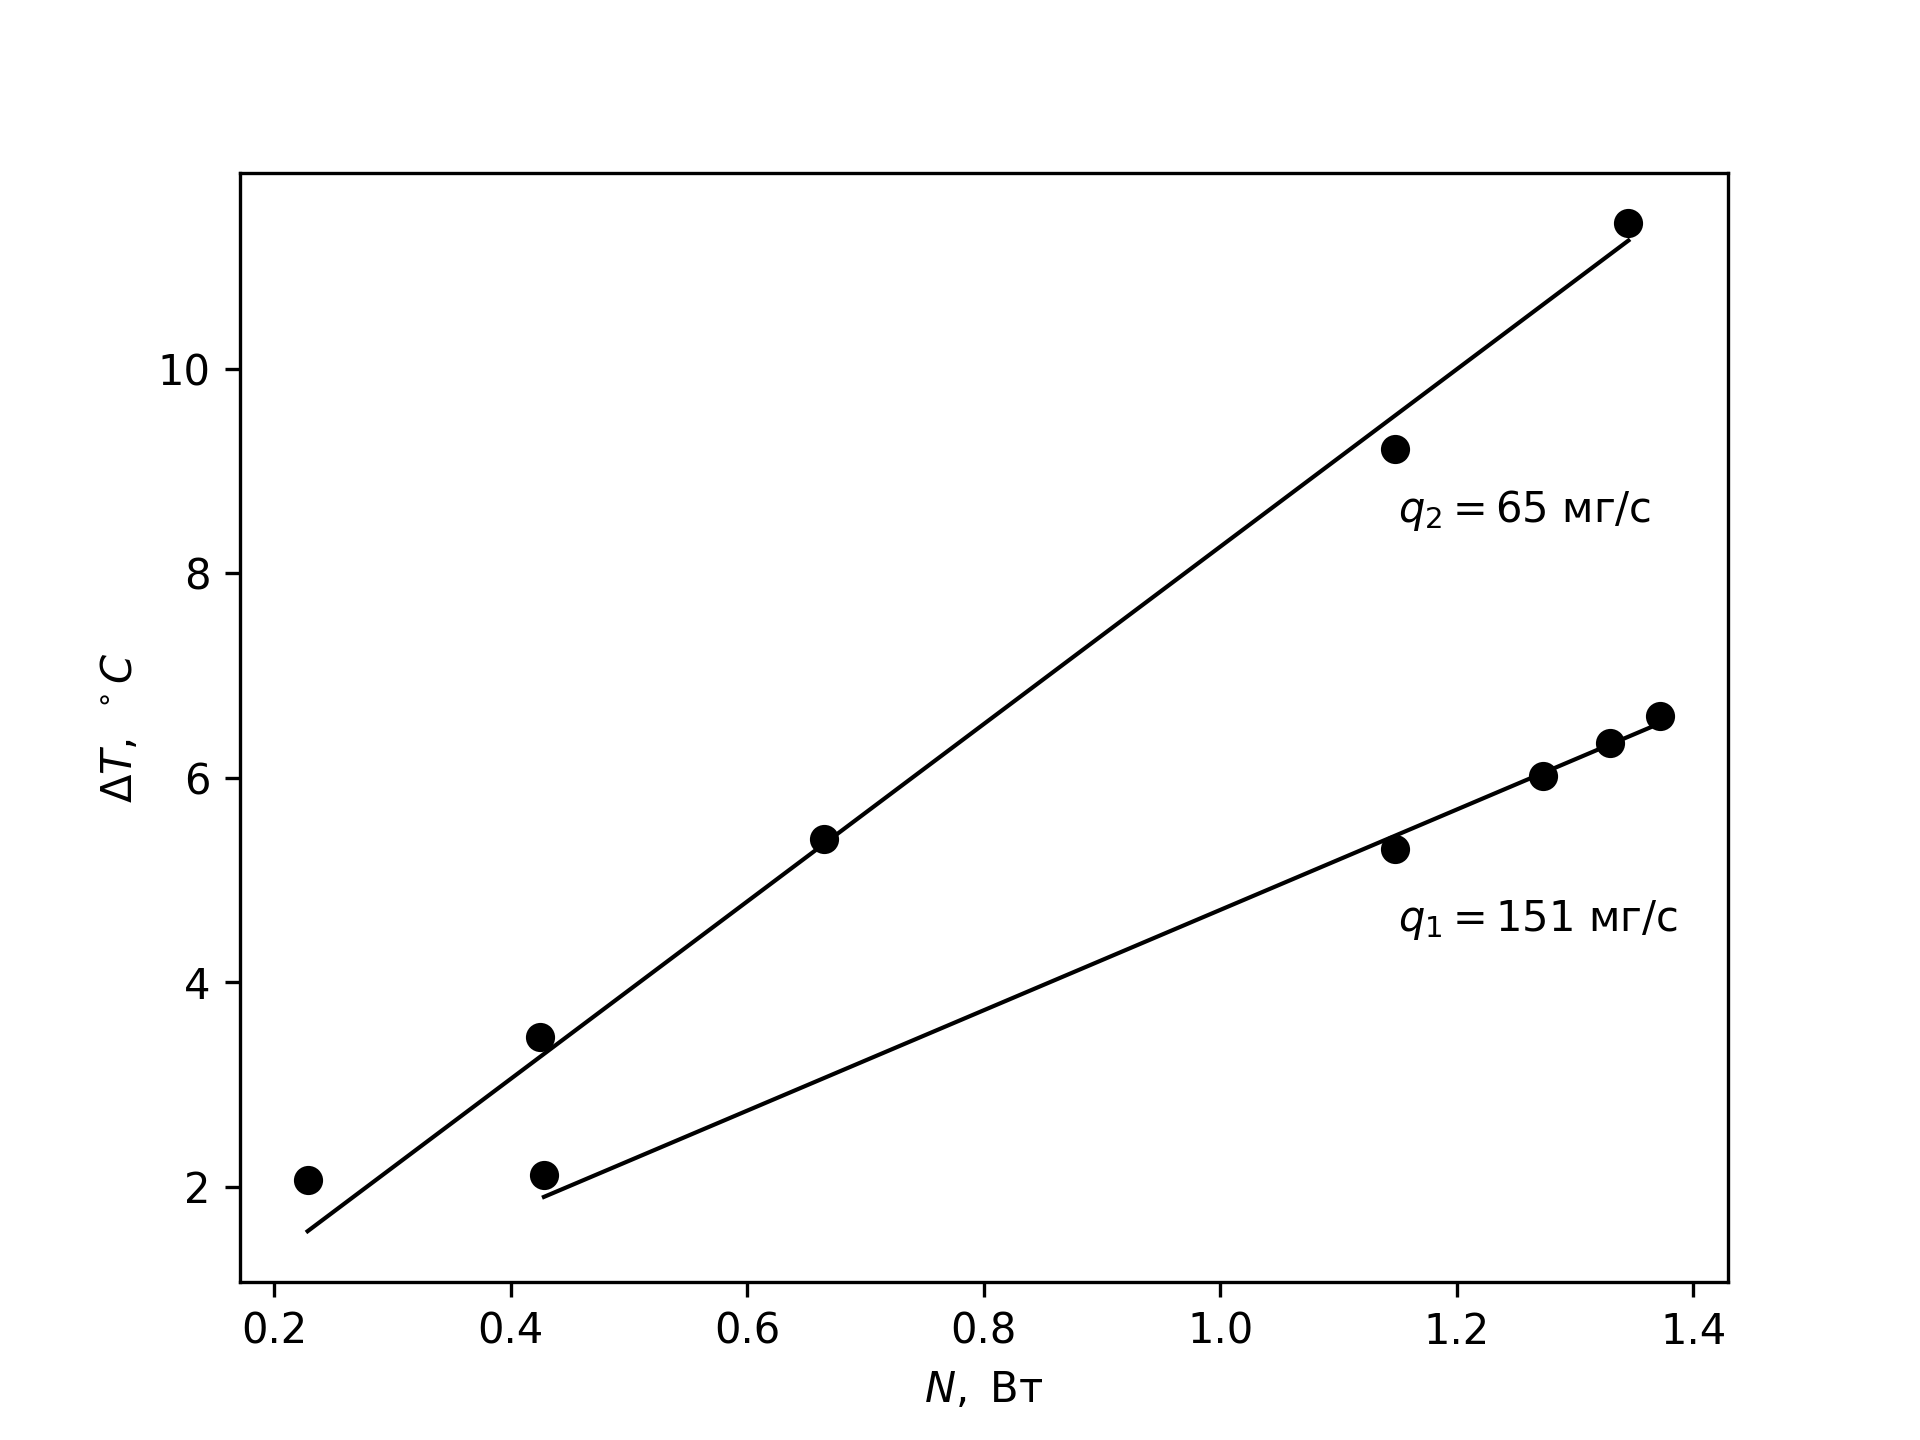
\includegraphics[scale=0.6]{terma8_1.png}
\caption{Зависимость $\Delta T(N)$ для различных значений $q$}
\end{figure}

\end{document}